\section{Durchführung}
\label{sec:Durchführung}
In diesem Versuch werden, wie in \autoref{sec:Ziel} bereits beschrieben, die Magnetfelder verschiedener Spulenkonstellationen gemessen. Die Messmethoden dazu werden im folgenden 
Kapitel erläutert. Zuerst werden jedoch die Vorbereitungsaufgaben diskutiert.
\subsection{Vorbereitungsaufgaben}
\label{subsec:VBA}
In der ersten Vorbereitungsaufgabe sollte die magnetische Flussdichte im Zentrum eines Helmholtzspulenpaares berechnet werden. Dies geschieht nach \autoref{eqn:Helmholtz}.
Die Spulen des Helmholtzspulenpaares haben einen Durchmesser $d = 125\unit{\milli\metre}$, der Abstand der Spulen beträgt $x = \sfrac{d}{2}$ gilt. Das Spulenpaar 
wird von einem Strom mit $1 \: \unit{\ampere}$ durchflossen. Mit diesen Werten und der magnetischen Feldkonstante 
$\mu_0 = 1.2566\cdot 10^{-6} \unit{\newton\per\ampere\squared}$\cite{scipy} ergibt sich $B(0) = 0.71\unit{\milli\tesla}$ für das Magnetfeld. 

Im zweiten Teil der Vorbereitung sollten die Begriffe Dia- Para- und Ferromagnetismus erklärt werden. 
\subsubsection{Diamagnetismus}
\label{subsubsec:DIA}
Diamagnetische Stoffe sind durch eine Permeabilität $\mu_{\text{r}} < 1$ ausgezeichnet. Liegt ein äußeres Magnetfeld an, bilden sie ein Gegenfeld, welches das anliegende Magnetfeld
abschwächt. Ohne äußeres Magnetfeld sind diamagnetische Stoffe nicht magnetisch. 
\subsubsection{Paramagnetismus}
\label{subsubsec:PARA}
Paramagnetische Stoffe verhalten sich gegenteilig. Sie sind ebenfalls ohne äußeres Magnetfeld nicht magnetisch, aber erzeugen in einem äußeren Magnetfeld ein paralleles Feld.
Die Felder überlagern sich, was zur Folge hat, dass das Gesamtfeld im Inneren des paramagnetischen Materials verstärkt wird. Paramagnetische Stoffen zeichnen sich durch eine 
Permeabilität $\mu_{\text{r}} > 1$ aus. 
\subsubsection{Ferromagnetismus}
\label{subsubsec:FERRO}
Ferromagnetische Stoffe können ohne ein äußeres Magnetfeld eigene permanente Magnetfelder besitzen. Diese bilden sich, da die einzelnen Atome jeweils magnetische Momente besitzen, welche 
dazu neigen, sich parallel zueinander auszurichten. Die ferromagnetischen Stoffe, die kein Magnetfeld besitzen, werden meist sehr stark von einem äußeren Pol angezogen. Solche Stoffe 
sind durch eine Permeabilität $\mu_{\text{r}} >> 1$ gekennzeichnet. Eine weitere wichtige Eigenschaft solcher Stoffe ist, dass sie sich magnetisieren lassen. Diese Magnetisierung findet
durch ein äußeres Magnetfeld statt und bewirkt, dass ein ferromagnetischer Stoff sein eigenes Magnetfeld aufbaut oder verändert. Hysteresekurven, wie zum Beispiel die in \autoref{fig:PlotHysterese},
geben die Magnetisierung gegen eine gewisse Größe an. In diesem Fall wird sie gegen den Strom angegeben.
\subsection{Messung des Magnetfeldes einer langen Spule}
\label{subsec:D_Lange_Spule}
Zur Messung des Magnetfeldes einer langen Spule benötigt man die Spule selbst, eine logitudinale Hall-Sonde und ein Netzgerät. Zunächst wird die Spule an das Netzgerät angeschlossen.
Dieses wird dann so eingestellt, dass die Spule von circa $1 \unit{\ampere}$ durchflossen wird. Anschließend wird die Hallsonde in einem Gestell befestigt, sodass die Messung 
möglichst auf einer Achse erfolgt.
Es wird ein Messnullpunkt festgelegt und die Sonde langsam in die Spule eingeführt. Dabei wird die relative Auslenkung zum Messnullpunkt und die Magnetfeldstärke 
an verschiedenen Stellen gemessen. Aus Symmetriegründen reicht es aus, bis zur Mitte der Spule zu messen.
\begin{figure}
    \centering
    \caption{In diesem Bild ist die verwendete lange Spule abgebildet. Die Länge der Spule wurde graphisch auf $16.4 \: \unit{\centi\metre}$ bestimmt.}
    \label{fig:Aufbau_lange_Spule}
    \includegraphics[width=0.7\textwidth]{content/LangeSpule.jpg}
\end{figure}
\subsection{Messung des Magnetfelds eines Spulenpaares}
\label{subsec:D_Spulenpaar}
Für diese Messung wird ein Helmholtzspulepaar benötigt, dessen Abstand variiert werden kann. Außerdem wird eine transversale Hall-Sonde zur Messung des Magnetfeldes benötigt. Zunächst
werden die beiden Spulen in Reihe an ein Netzgerät angschlossen, sodass beide Spulen gleichsinnig vom Strom durchflossen werden. Nun wird ein Abstand zwischen den Spulen 
festgelegt. Die Hall-Sonde wird, wie in \autoref{fig:Aufbau_Spulenpaar} dargestellt ist, in eine Führungsschiene eingesetzt. Dadurch ist garantiert, dass stets entlang einer Achse
gemessen wird.
Anschließend werden Wertepaare der Position auf der Achse und der magnetischen Flussdichte in sinnvollen Abständen notiert. Dabei wird sowohl der Bereich zwischen den Spulen, 
als auch der Bereich außerhalb der Spulen gemessen. Dies wird für drei unterschiedliche Abstände der Spulen wiederholt.
\begin{figure}
    \centering
    \caption{In diesem Bild ist der Versuchsaufbau zum Helmholtzspulenpaar dargestellt.\cite{v308}}
    \label{fig:Aufbau_Spulenpaar}
    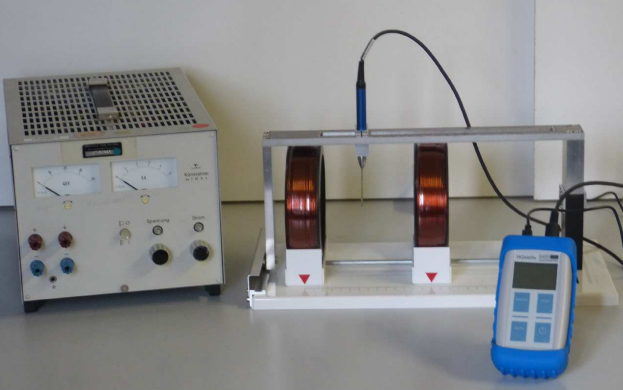
\includegraphics[width=0.7\textwidth]{content/HelmHoltzAufbau.PNG}
\end{figure}
\subsection{Messung des Magnetfeldes einer Toroid-Spule zur Bestimmung der Hysteresekurve}
\label{subsec:D_Hysterese}
Für diese Messung wird eine Toroidspule und eine transversale Hall-Sonde benötigt. Die Hall-Sonde wird über eine Vorrichtung in den Luftspalt der Toroidspule gehalten. Die Toroidspule
wir an ein Netzgerät angeschlossen. Bevor dieses eingeschaltet wird, muss die Spule ausreichend gut entmagnetisiert werden. Nun wird der Strom
der Spule langsam hochgeregelt, wobei die dazugehörigen Feldstärken notiert werden. Es bietet sich an, eine Schrittweite von $1 \: \unit{\ampere}$ zu wählen. Es wird gemessen bis die 
gesamte Hysteresekurve abgemessen wurde. Dies bedeutet, dass die Stromstärke bis zu einem Wert von $10 \: \unit{\ampere}$ erhöht wird und anschließend stückweise verringert wird, bis
wieder $0 \: \unit{\ampere}$ eingestellt sind.
Um die Messung im negativen Bereich fortzusetzen, wird die Verkabelung gegenpolig angeschlossen. Der zuvorige Messprozess wird für die negative Polarität wiederholt. 
Zuletzt werden die Kabel wie zu Anfang angeschlossen und bis zu einer Stromstärke von $10 \: \unit{\ampere}$ gemessen.
\begin{figure}
    \centering
    \caption{Dies ist ein Bild des Versuchaufbaus zur Toroidspule.\cite{v308}}
    \label{fig:Aufbau_Toroid}
    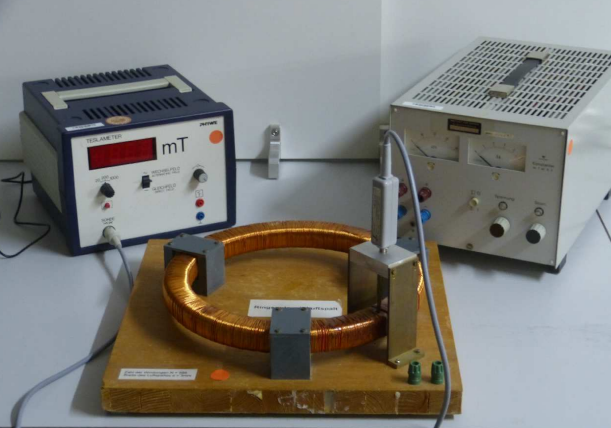
\includegraphics[width=0.7\textwidth]{content/RingSpuleAufbau.PNG}
\end{figure}